\def\theTopic{Peanut Allergies}
\def\dayNum{12 }

\begin{center}
{\bf {\large Peanut Allergies}}
\end{center}
\vspace{-.1in}

Peanut allergies are so common in children that all parents have to
closely watch the snacks they bring to an elementary classroom party. 
Any hint of peanuts in a cookie can endanger some kids. A recent
article suggests that peanut allergies can be prevented by giving
babies (ages 4 to 10 months) some peanut protein every week until they
are 5 years old. They randomly divided 500 infants into ``Eat
peanuts'' and ``avoid peanuts'' groups and followed them to age five
when each child was checked for peanut allergies.

The researchers want to answer this question:
\begin{center}
  {\large\sf  Does feeding children peanut protein prevent peanut allergies?} 
\end{center}
{\bf
Discuss the Following Questions	}

\begin{enumerate}
  \item  Is there a treatment condition in this study? (If so, what?)
\begin{students}
\vspace{2cm}
\end{students}

\begin{key}
  {\it Yes, feeding an infant 6 g per week of peanut protein or avoiding
    peanut protein. }
\end{key}


  \item  What is the response variable in this study?
\begin{students}
\vspace{2cm}
\end{students}

\begin{key}
  {\it  Peanut Allergy at age 5 years. }
\end{key}

  \item  Are the variables above quantitative or categorical?
\begin{students}
\vspace{2cm}
\end{students}

\begin{key}
  {\it  Both are categorical. }
\end{key}


Results: 5 of the 245 infants getting peanut protein,  (2\%)  showed
allergic symptoms to peanuts, whereas in the peanut
avoidance group, 35 (13.7\%) of 255 infants developed allergic
symptoms to peanuts. (BTW, the two groups started with equal, somewhat
larger numbers of infants, but there were dropouts who are assumed
ignorable. )


  \item \label{PnutTable} Organize the results into a 2 by 2 table
\begin{students}

{\Large
    \begin{tabular}[c]{|l|c|c|c|} \hline
        &Peanuts (1) & Avoiders (2) & total \\ \hline
Allergic    &   &   & \\ \hline
Not Allergic&   &   & \\ \hline
Total & & & \\ \hline
    \end{tabular} \vspace{1cm}
}
\end{students}
\begin{key}

\begin{tabular}[c]{|l|c|c|c|} \hline
        &Peanuts & Avoiders & total \\ \hline
Allergic& 5  & 35  &  40\\ \hline
Not Allergic& 240  &  220 &460 \\ \hline
Total & 245  &  255 & 500\\ \hline
\end{tabular}
\end{key}

\item Of the 245 subjects assigned to the eat peanuts, what proportion
  improved? We will label this 
     $\widehat{p}_1$ because it is an estimate of $p_1$,  the true proportion
     who would become allergic if all infants ate peanut protein.  As
     in the notes for Activity 4,  we ornament $p$ with a ``hat'' on top to
     show that this is an estimate (or 
     a statistic) computed from the observed sample.  Finally, the ``1''
     subscript is to demark the first (treatment) group.
\begin{students}
\vspace{2cm}
\end{students}

\begin{key}
  {\it $\widehat{p}_1 = 5/245 = 0.02$ }
\end{key}



   \item  Of the 255 subjects assigned to the control condition, what
     proportion improved? We'll call this $\widehat{p}_2$, using a ``2''
     for the control group. 
\begin{students}
\vspace{2cm}
\end{students}

\begin{key}
  {\it  $\widehat{p}_2 = 35/255 = 0.137$}
\end{key}



   \item Find the difference between the proportion of subjects
     assigned to the ``eat peanuts'' condition that became allergic and the
     proportion of subjects assigned to the control condition that
     became allergic.  $\widehat{p}_1 - \widehat{p}_2$ = 
\begin{students}
\vspace{2cm}
\end{students}

\begin{key}
  {\it  $0.02 - 0.137 = -0.117$}
\end{key}

   \item What proportion of all 500 subjects improved?  This is called
     a marginal distribution because it just uses totals.  If the
     treatment has no effect, then this will be a good estimate of the
     true overall probability that any infant will develop peanut
     allergy, so label it $\widehat{p}_T$ where $T$ goes with ``Total''.
\begin{students}
\vspace{2cm}
\end{students}

\begin{key}
  {\it $\widehat{p}_T = 40/500 = 0.08$ }
\end{key}


   \item  Write a few sentences summarizing the results in the
     sample. This summary should include a summary of what the data
     suggest about: (1) the overall risk of becoming allergic to
     peanuts in these  subjects; (2) the differences between the two
     treatment groups; 
     and (3) whether or not the data appear to support the claim that
     peanut eating is effective. 
\begin{students}
\vspace{4cm}
\end{students}

\begin{key}
  {\it       The data suggests that overall approximately 8\% of
     participants developed peanut allergies, but the difference
     between the proportions who became allergic in the two treatment
     groups  was -11.7\%.  This appears to be a large difference which
     supports the idea that eating peanuts early helps infants avoid
     peanut allergies.}
\end{key}

   \end{enumerate}
   
   In statistics, we use data from a sample to generalize back to a
   population.  Here are some {\bf critical questions}:
   \begin{itemize}
   \item Does the higher allergy rate in the control group provide
     convincing evidence that the peanut eating is effective?
   \item Is it possible that there is no difference between the two
     treatments and that the difference observed could have arisen
     just from the random nature of putting the 500 subjects into
     groups (i.e., the luck of the draw)?
   \item Is it reasonable to believe the random assignment alone could
     have led to this large of a difference?
   \item Just by chance did they happen to assign
     more of the subjects who were going to improve into the peanut
     treatment group than the control group?
   \end{itemize}
 
   One way to examine these questions is to consider what you would
   likely see if 
   40 of the 500 kids were going to develop the allergy (the number of
   infants  who did in our sample) regardless of whether they ate
   peanuts or not. If that is the case, you would have expected, on
   average, about 20 of those subjects to end up in each group
   (the null model suggests this). 

   We will answer this question by using a web applet to conduct a
   {\bf permutation} (or randomization) test which lets us see the
   results one can get just due to variation in random
   assignment. We'll operate under the null model assumption that the
   control and peanut conditions have no effect on developing a peanut
   allergy.  With two proportions, we use   $$H_0: p_1 = p_2$$

   Note: hypotheses are always about parameters. Never use a ``hat''
   on the $p$'s in the hypothesis.  As before, the direction of the
   alternative depends on what the research is intended to show: no
   difference (could go either way, so use $\neq$), less than, or
   greater than.  You must specify which proportion is being
   subtracted from the other, because it will change the direction of
   the alternative.
 
   The term ``permutation'' just means that we are mixing up, or
   permuting, the group assignments.  In physical terms, it's
   shuffling the cards and redealing them into two groups.  Because
   this is a randomized experiment, it's also fine to call this a
   ``randomization'' test.  We are looking at what might have happened
   if treatments were equally effective, and we reassigned individuals
   to (possibly different) groups.

 \begin{enumerate}
  \setcounter{enumi}{9}
 
   \item  The null hypothesis is: $H_0:\  p_1 = p_2$  or $H_0:\  p_1 -
     p_2 = 0$ or $p_{treat} =   p_{control}$. Is the researcher's question looking
     for an increase, decrease, or change in either direction?  Fill
     in the blank with $<$, $>$, or $\neq$ for the alternative
     hypothesis:  

\begin{students}
     $H_A:  p_{treat}$  \underline{\hspace{2cm}}   $p_{control}$
\end{students}
\begin{key}
   $H_A:  p_{treat} < p_{control}$
\end{key}     

   Go to the  web page:
   \url{http://shiny.math.montana.edu/jimrc/IntroStatShinyApps/}
   and select ``Enter Data'' under  \underline{\sf 2 Categ}.
   Enter the numbers and labels from the table in \ref{PnutTable}.
   The proportions should agree with those above, but let's check:
   \begin{enumerate}
   \item 
     The proportion of infants in Peanut group who became allergic: \\ 
\begin{key}
 0.02       
\end{key}
   \item The proportion of infants in Control group who became allergic: \\ 
\begin{key}
 0.137       
\end{key}
\item The difference in proportions between the two groups: 
\begin{students}
\vspace{2cm}
\end{students}

\begin{key}
  {\it $ \pm 0.117$ }
\end{key}
\end{enumerate}


   \item  Click ``Test'' under ``2 categ.'', and generate  1000
     shuffles and sketch the plot below. 
\begin{students}
\vspace{4cm}
\end{students}

\begin{key}
  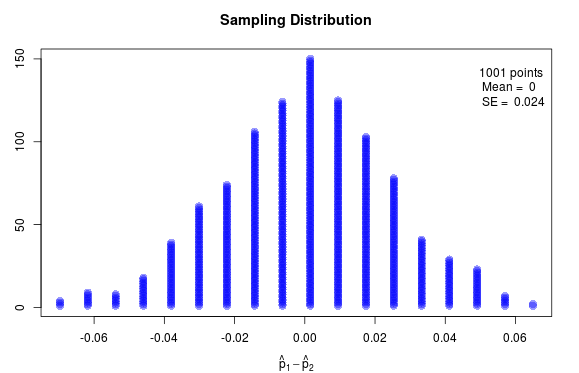
\includegraphics[width=.6\linewidth]{../../plots/peanutTest-1000.png}
\end{key}

% \item  If you click on a bar in the histogram, you should see a small
%   dark rectangle, and the blue/green splits will change between
%   bars. What does one rectangle in a bar represent?
% \begin{students}
% \vspace{3cm}
% \end{students}

% \begin{key}
%   {\it      Each rectangle represents a single re--randomized trial in with the
%      13 improved participants were randomly assigned to one of the
%      two treatments.  The location of its bar gives the difference
%      in the proportions of improved subjects in each group (dolphin therapy --
%      control).  }
% \end{key}

   \item  Where is the plot of the results centered (at which value)?
     Explain why this makes sense. 
\begin{students}
\vspace{2cm}
\end{students}

\begin{key}
  {\it       It is centered at 0 because 
     the null hypothesis is that the treatment has no effect on
     allergy development in which case we should see the same proportion of
     allergic kids in both groups (or the difference in
     proportions should be 0). We are assuming $H_0$ is true. }
\end{key}

   \item  
     Report the approximate p--value (i.e., strength of evidence) based
     on the observed result. (Reminder: we did this in the helper --
     hinderer study on Activity 6.)
\begin{students}
\vspace{1cm}
\end{students}

\begin{key}
  {\it  I got $0/10000 < 0.0001$}
\end{key}

       Go back to \fbox{Enter Data} and change labels slightly to clear
       the plot and then  generate 
       another 5000 random shuffles. How  much does the strength of
       evidence change?
\begin{students}
 \vspace{1cm}
\end{students}

\begin{key}
  {\it I got $63/5000 =0.0126$. Little to no change. }
\end{key}
\vspace{1cm} 


    \item  Based on the p--value, how strong would you consider the
      evidence against the null model?  
\begin{students}
\vspace{1cm}
\end{students}

\begin{key}
  {\it    strong}
\end{key}


 
    \item  Based on the p--value, provide an answer to the research
      question.  
\begin{students}
\vspace{2cm}
\end{students}
\begin{key}
  {\it        With a p--value of 0.001, there is very  strong evidence to
      reject the null hypothesis.  We can conclude that in the
     group of infants from which these were drawn, eating peanut
     protein as an infant caused a reduction in prevalence of peaut
     allergy as evidenced by a lower proportion
      of allergic kids in the treatment group over the
      control group. }
\end{key}

    \item   Another study on the effects of a different therapy had a
      p--value of 0.25.  How would you report those results? 
\begin{students}
\vspace{3cm}
\end{students}

\begin{key}
  {\it       With a p--value of 0.25, there is little to no evidence
      against the null hypothesis.  We cannot conclude that
      swimming with dolphins is therapeutic for patients suffering
      from depression.  }
\end{key}



    \item  A third study computed p--value to be 0.73. How would you
      report those results?   
\begin{students}
\vspace*{4cm}
\end{students}

\begin{key}
  {\it        With a p--value of 0.73, there is  no evidence
      against the null hypothesis.  We cannot conclude that
      swimming with dolphins is therapeutic for patients suffering
      from depression. }
\end{key}


    \item \label{reportBullets} Write up  the pertinent
      results from the analysis on your own paper. When reporting the
      results of a permutation test, pertinent information from the
      analysis that  needs to be included is: 
      \begin{itemize}
      \item The type of test used in the analysis (including the
        number of trials [shuffles]);
      \item The null model assumed in the test;
      \item The observed result based on the data;
      \item The p--value and strength of evidence of the test and your
        conclusion; and
      \item The appropriate scope of inference based on the p--value
        and the study design.  Include:
        \begin{itemize}
        \item How were the subjects selected?  If they are a random
          sample from some population, then our inference goes back to
          the population.
        \item Were treatments assigned?  If treatments were assigned
          at random, then we can state a causal conclusion.
        \end{itemize}
      \end{itemize}
\begin{key}
 {\it      A randomization test for a difference in proportions with
      5000 trials was used to test the null hypothesis that eating
      peanut protein has no effect on whether or not an infant will
      develop peanut allergy.  In 500 participants randomly split 
      into 245 treated and 255 control babies, 40 developed peanut
      allergies: 5 in the treatment group and 35  in the control
      group.  This gave an observed difference in
      proportion of allergic kids between the treatment and
      control group of -0.117 (peanut proprotion minus control).  This
      resulted in a p--value of $< 0.0001$, which constitutes  strong
      evidence against the null hypothesis.  Since participants
      were randomly assigned to groups and are representative 
      of all infants in the UK, we can
      conclude that in all UK babies, eatingpeanuts caused a lower
      proportion of infants to develop a peanut allergy as compared to a
      control group.   
     }  
\end{key}

\end{enumerate}

\newpage
\begin{center}
  {\bf Take Home Messages}
\end{center}
  \begin{itemize}
  \item We are conducting a permutation test which simply mixes up the
    labels.  Because of random treatment assignment, this is also a
    randomization test. 
  \item We tested to see if  two proportions were
    equal. This is much like what we did in Unit 1 with a single
    proportion, except that the null hypothesis states that the two
    population proportions are equal (instead of one proportion coming
    from ``blind guessing'').
  \item Question \ref{reportBullets} asks you to write up results.
    Communicating 
    and reading statistical results is a very important skill.  We
    will keep doing this though the rest of the semester.  We hope you
    can dive right into the task, but if you have any questions,
    please ask.  You need to get this skills down -- the sooner the
    better. 
 \item 
 Any questions?
  \end{itemize}



